% \chapter*{\centering{\large{LEMBAR PENGESAHAN}}}
% \thispagestyle{empty} {\bf }Dengan ini saya mahasiswa Fakultas
% Matematika dan Ilmu Pengetahuan Alam, Universitas Negeri Jakarta

% \vskip3mm

% \begin{tabular}{ll}
%   Nama & : Akbar Maulana Alfatih \\
%   No. Registrasi & : 1313619003\\
%   Program Studi & : Ilmu Komputer \\
%   Judul & : Rancang Bangun Aplikasi Teknologi Perikanan Modern \\ & \hspace{0.2cm}  Dengan Fitur Inventarisasi Berbasis Multi Platform \\
% %  Judul & : Pengaruh Penggunaan \emph{Color Model} LAB dan HLS dalam \\ & \hspace{0.2cm} Kalibrasi Warna Luka Menggunakan Metode Segmentasi \\ & \hspace{0.2cm} \emph{K-Means} dan \emph{Mean Shift}\\
% \end{tabular}

% \vskip3mm

% \noindent \hskip10mm Menyatakan bahwa proposal skripsi ini telah siap diajukan untuk seminar pra skripsi.
% %\begin{center}
% %Menyatakan bahwa skripsi ini telah siap diajukan untuk sidang skripsi.
% %\end{center}



% \begin{center}
% \vskip3mm

% Menyetujui,

% \vskip3mm
% \begin{spacing}{1.25}

% \begin{tabular}{ccc}
%   \hskip-2mm Dosen Pembimbing I & \qquad \qquad \qquad \qquad & \hskip-6mm Dosen Pembimbing II \\
%    &  &  \\
%    &  &  \\
%    &  &  \\
%    &  &  \\
%   \hskip-2mm \underline{\textbf{Muhammad Eka Suryana, M. Kom}} &  & \hskip-6mm \underline{\textbf{Med Irzal, M.Kom.}} \\
%   \hskip-2mm NIP. 19851223 201212 1 002 &  & \hskip-6mm NIP. 19770615 200312 1 001	 \\
% \end{tabular}
% \end{spacing}
% \end{center}
% \vskip3mm
% \begin{center}
% Mengetahui, \\
% Koordinator Program Studi Ilmu Komputer
% \end{center}
% \begin{spacing}{1.25}
% { \ }
% \\
% \\
% { \ }\begin{center}
% \underline{\textbf{Ir. Fariani Hermin Indiyah, M.T.}} \\
% {NIP. 19600211 198703 2 001}
% \end{center}
% \end{spacing} 
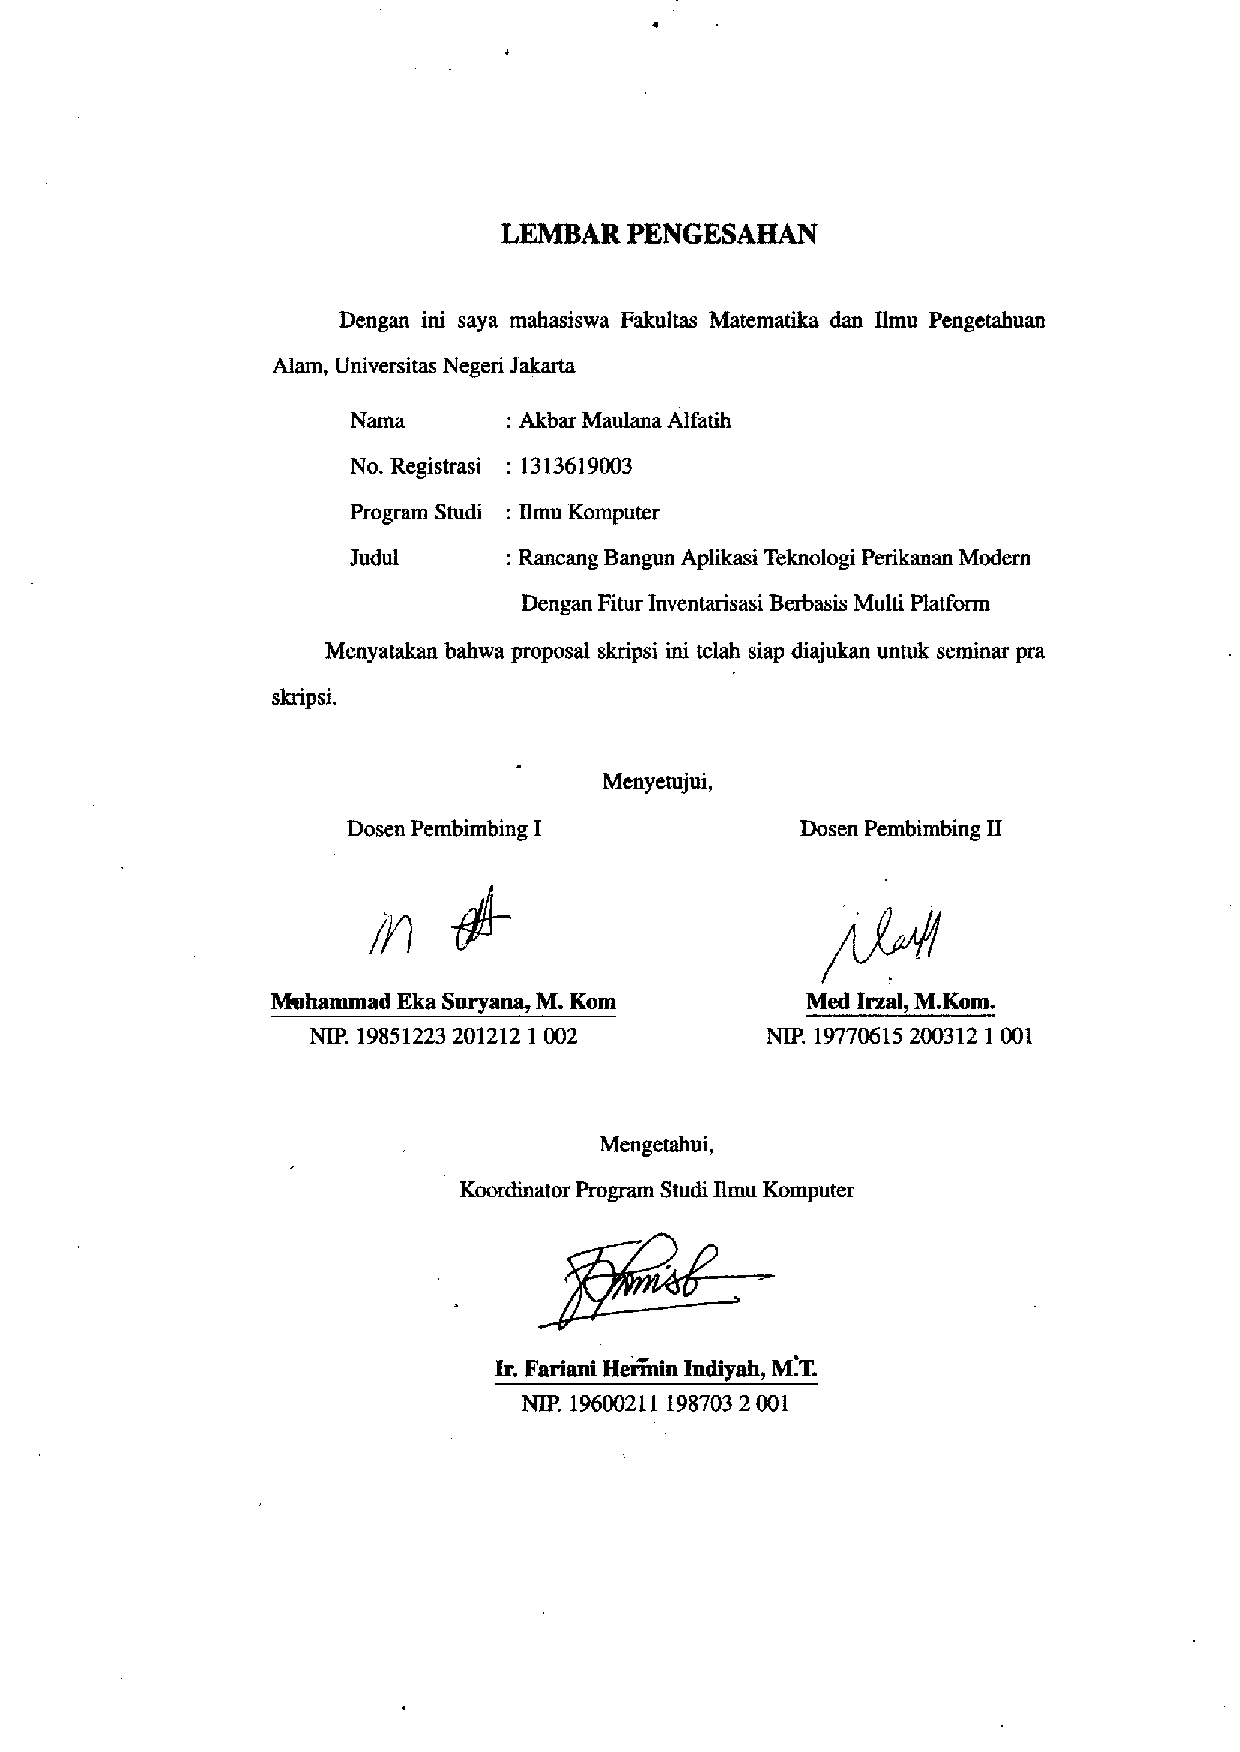
\includepdf[pagecommand={\thispagestyle{plain}},
  pages=1]{assets/lembar_pengesahan_sps.pdf}